\documentclass[12pt]{article}
\usepackage[margin=1in]{geometry}
\usepackage{physics}
\usepackage{graphicx}
\usepackage{fontspec}
\setmainfont{Times New Roman}
\setmonofont{Courier}

\usepackage{hyperref}
\hypersetup{
    colorlinks=true,
    linkcolor=blue,
}
\renewcommand{\d}{\mathrm d}
\newcommand{\I}{\mathrm i}
\newcommand{\e}{\mathrm e}
\usepackage[varg]{newtxmath}

\title{Comic Book Movies Affecting Comic Book Sales \vspace{0.5em}\\ \Large Final Report for PHY 408}
\date{\today}
\author{Jack Farrell \\ 1003978840}

\begin{document}
\maketitle
\tableofcontents
\pagebreak
\section{Introduction}
In the last two decades, movies based on comic books have become some of the most popular in Hollywood.  On the other hand, due in part to a speculative boom leading to a crash\footnote{Very interesting --- see \textit{e.g.} \hyperlink{https://www.washingtonexaminer.com/weekly-standard/the-crash-of-1993}{https://www.washingtonexaminer.com/weekly-standard/the-crash-of-1993}} and in part due to the emergence of digital media, the sales of comic books themselves have declined from their peak values in the 1990s.  In theory, the enormous success of the super-hero genre on the big screen should translate to increased interest in the comic book source material.  Determining the extent to which this link exists is the focus of our project.

In this report, we use Fourier Transforms and the $cross-correlation$ of two time series to analyze the total monthly earnings of comic books and comic book movies, and their relationships. We limit out focus to movies in the \textit{Marvel Cinematic Universe (MCU)}, a collection of films featuring comic book characters like \textit{Iron Man}, \textit{Thor}, \textit{Captain America}, and \textit{Spider-Man}.  These projects feature somewhat faithful adaptations of comic-book characters and stories, and they also represent some of the most profitable and successful comic-book movies, with over 22 Billion (USD) box-office earnings worldwide.

Our analysis is guided by the question: \textbf{To what extent do the releases of MCU films affect the sales of Marvel comic-books?}  We hypothesize the following: on one hand, on a broad scale, the prevalence of Marvel adaptations during the time period of the MCU's activity should cause a general upward trend of Marvel comic-book sales.  Additionally, though, fluctuations in comic-book sales around the broad trends should be correlated with the release of MCU movies.

\section{Analysis}
\subsection{Data Sources}
This project takes data from two sources.  For the comic book sales figures, we pull from ``Comichron" (\hyperlink{https://www.comichron.com/}{https://www.comichron.com/}), an internet database featuring monthly comic book sales figures.  For the movie earnings, we pull from ``Box Office Mojo" (\hyperlink{https://www.boxofficemojo.com/}{https://www.boxofficemojo.com/}), an internet database giving various data related to movies, including box-office earnings over time.


\subsection{Raw Data}
We focus on the \textit{total} earnings of all comics published by Marvel and the \textit{total} earnings of all movies in the MCU ---  in other words, we analyze the general relationships between Marvel movies and Marvel comics holistically.  The reason for this choice is that the sales of individual series of comics (\textit{e.g. The Amazing Spider-Man}) are volatile and change with many factors including the writer and artist. On the other hand, we expect the publisher-wide sales figures to depend on less variables.  Our datasets cover all months between Jan. 2008 and Dec. 2019, roughly bookending the MCU (so far!).

Fig. (\ref{fig:raw_data1}) plots the total Marvel Comics earnings over the MCU's history (again, 2008--2019 inclusive).
\begin{figure}[h]
    \centering
    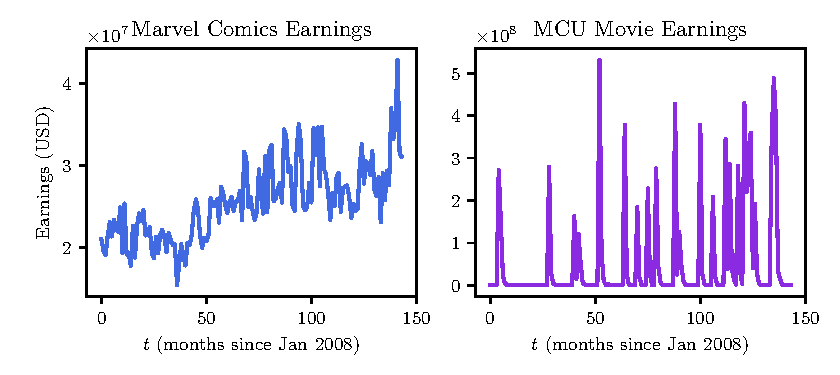
\includegraphics{figures/raw_data1.pdf}
    \caption{\textit{Left panel} Total Marvel Comics earnings as a function of time $t$ in months since Jan. 2008.  \textit{Right panel} Total Marvel Cinematic Universe domestic box office earnings as a function of time $t$ in months since Jan. 2008.}\label{fig:raw_data1}
\end{figure}
As we might expect, the MCU dataset (purple trace, right panel) shows a constant zero signal interrupted by sharp peaks corresponding to the release of movies.  On the other hand, the comics data shows a broad complicated trend with superimposed high-frequency fluctuations.  Our first step will be to filter the data to convince ourselves that there really is a trend.


\subsection{Filtering}
\label{sec:filtering}
To make the trend more clear, we filter the data.  First, we estimate the trend using a least-squares fit to a degree 5 polynomial.  We used the \texttt{numpy.polyfit()} function.  Then, we subtract the trend, leaving just the fluctuations around the estimated trend.  We give the raw data, trendline, and detrended data in Fig.~(\ref{fig:detrended1}).
\begin{figure}[ht]
    \centering
    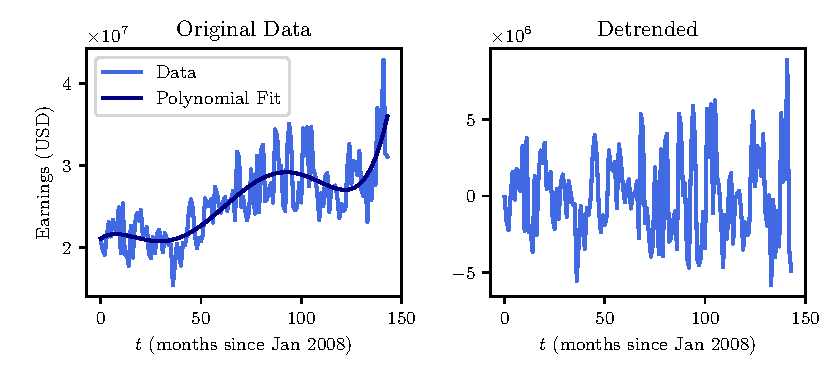
\includegraphics{figures/detrended1.pdf}
    \caption{\textit{Left panel} Raw comic book earnings and a degree 5 polynomial fit.  \textit{Right panel} Subtracting the polynomial trendline from the raw data to obtain a `detrended' time series.}\label{fig:detrended1}
\end{figure}
Then, we filter the data using the \textit{Fourier Transform} of our time series $f$, defined by:
\begin{equation}
    F_k = \Delta t \sum_{j=0}^{N-1}f_j \e^{-\I 2 \pi j k}.
\end{equation}
We plot the Fourier Transform in Fig.~(\ref{fig:fourier}).
\begin{figure}[ht]
    \centering
    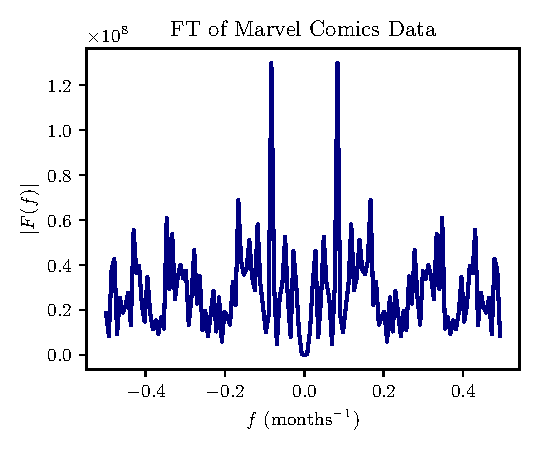
\includegraphics{figures/fourier.pdf}
    \caption{Amplitude of the fourier transform of the Marvel Comics Earnings time series as a function of frequency $f$.}\label{fig:fourier}
\end{figure}
Based on the amplitude of the peaks, which give roughly the `component' of the signal that has the corresponding frequency, we find the highest amplitude peaks have frequencies lower than $0.1$ month$^{-1}$ in absolute value.  As such, to smooth out the data, we set all Fourier components corresponding to frequencies greater than that value to zero, effectively truncating our Fourier Transform.  Taking an inverse Fourier Transform and adding back in the polynomial trend, we obtain the smoother trace shown in Fig.~(\ref{fig:filtered}).
\begin{figure}[h]
    \centering
    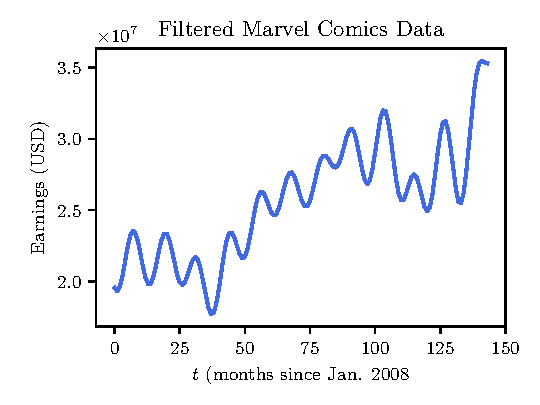
\includegraphics{figures/filtered.pdf}
    \caption{Result of filtering the Marvel Comics data by truncating the Fourier Transform}\label{fig:filtered}
\end{figure}
As we expected because of the polynomial fit (and from eyeballing the raw data), there is a general upward trend over the course of out roughly ten-year window of analysis.  Interestingly, the increase seems to correspond with the \textit{number} of MCU releases, but we do not elaborate on the quantitative aspects of this relationship in this report, preferring instead the correlation analysis of the following subsection.


\subsection{Correlation}
\label{sec:correlation}
Having considered (briefly) the broad affects of increasing MCU releases on Marvel comics data in the form of showing the explicit trend in the latter, we now turn to studying \textit{fluctuations} around the general trend. In other words, we investigate the correlation between the MCU's earnings and the fluctuations of Marvel's comic book earnings relative to their general trend.  For this, the tool we use is the \textit{cross-correlation} between time series $f$ and $g$:
\begin{equation}
    C_{fg}(\tau) = \int_{-\infty}^\infty \d \tau f^*(t)g(t+\tau).
\end{equation}
Which, in roughly, gives the correlation between the two time series when $g$ is shifted by an amount $\tau$.  Peaks in $C_{fg}$ when it is graphed as a function of $\tau$ give the extent to which $g$ is related to $f$ when $g$ is shifted by an amount $\tau$.

We first detrended the data like shown in Fig.~(\ref{fig:detrended}).  We also normalized the resulting detrended data by dividing by the maximum (absolute value) entry.  We do the same for the MCU earnings data: making the two series more comparable in magnitude gives more reasonable values for the cross-correlation.

Then, with the two normalized datasets (and the comics series detrended), we compute the cross-correlation. Fig.~(\ref{fig:correlation1}) gives the cross-correlation between the MCU and Marvel Comics earnings time series.
\begin{figure}[h]
    \centering
    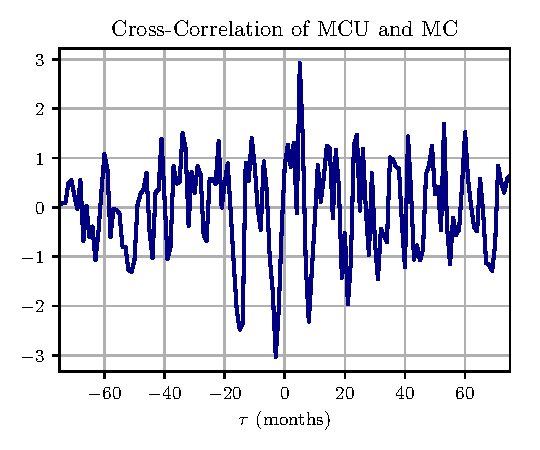
\includegraphics{figures/correlation1.pdf}
    \caption{Cross-correlation of the MCU earnings dataset and the Marvel Comics (MC) dataset as a function of $\tau$, the shift between the time series.  Peaks give region of high correlation.}\label{fig:correlation1}
\end{figure}
The $\tau-$axis is arranged a positive value of $\tau$ corresponds to shifting the comics time series (in the positive direction) by an amount $\tau$.  In general, the results are not conclusive: we do not notice any convincing peaks suggesting correlation.

Still, we can extract some weak information from the plot.  For instance, we do notice one peak that stands out at $\tau\approx 6$ months.  This peak means that the comic book data around 6 months \textit{earlier} is related to the MCU data.  This makes sense: for big-budget movies like those in the MCU, the advertising campaign for the films would start around this time, including the release of several `trailers' and television spots.  According to our analysis, it is the beginning of this process that affects comic book sales more than their actual release.  There is also a peak at $\tau = 0$, but it does not stand out from the backgorund noise in the plot.

\subsection{Control}
To make our claim more convincing, it helps to have a `control' dataset.  If our hypothesis is correct, the sales figures for publishers outher than marvel should not display the same behaviour at $\tau \approx 6$ months.  We choose ``IDW Publishing" --- while ``DC Comics"  may be a more obvious choice, it would not be a proper control given that its comics fall into the same genre as Marvel's.  Performing the same analysis described above on the monthly sales figures for IDW gives the results shown in Fig.~(\ref{fig:correlation2}).
\begin{figure}[h]
    \centering
    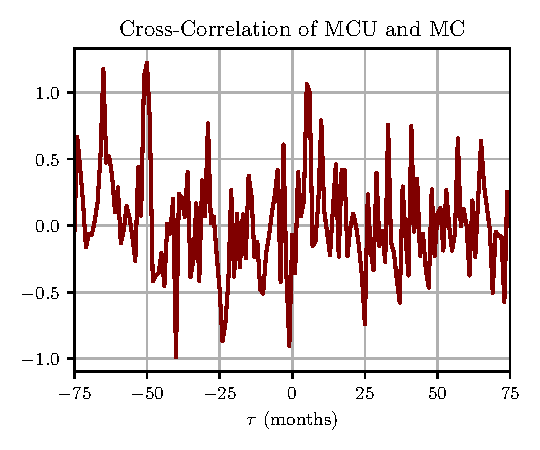
\includegraphics{figures/correlation2.pdf}
    \caption{Cross-correlation of the MCU earnings dataset and the Marvel Comics IDW Comics earnings dataset as a function of $\tau$, the shift between the time series.  Peaks give region of high correlation.}\label{fig:correlation2}
\end{figure}
Here, the noise is comparable even to the peak near $\tau \approx 5$, and there are even some stronger peaks near $\tau \approx -55$.  As such, we claim that the correlation peak we discussed in Sec.~(\ref{sec:correlation}) are ``real": it really does represent a fact about the affect of comic book movie advertising on comic book sales.

\subsection{Sources of Error}
\label{sec:sources_of_error}
The analyses described in the following three sections are subject to several errors.  To start, the noisiness of the data means that the peaks we identify in the cross-correlation are challenging to distinguish from the background.  While our analysis of the `control' dataset in the previous section makes the claims more plausible, the correlation is still not strong.  Secondly, the availability of higher-resolution (daily) comics earnings figures could, since it might be that the `spike` in comic book sales lasts for less than a month, and would thus get lost in our monthly data.



\section{Conclusion}
The analysis described in this report does not quite confirm or deny our hypothesis, nor give a convincing answer to our guiding question about the effects of comic book movies on comic book sales.  Still, we found two pieces of plausible evidence that certainly motivate future more sophisticated investigations into this topic.  First, in Sec.~(\ref{sec:filtering}), we found that filtering the monthly comic book sales data revealed a strong visual connection between the broad increase in comic book sales over our ten-year window of study and the release of MCU films over the same period.  Even more convincingly, in Sec.~(\ref{sec:correlation}), using techniques involving the cross-correlation, we obtain results suggesting that the lead-up to releasing MCU films (advertising campaigns, plausibly) does measurably affect comic book sales.

The outcomes of this study give us several ideas for future projects.  Two main directions stand out.  First, it would be interesting to perform a similar analysis using \textit{all} comic films compared to \textit{all} super-hero comic books --- we might find an even stronger correlation.  Secondly, we could take the opposite approach, analyzing the sales figures of individual comic-book series compared with specific film franchises (\textit{e.g.} Avengers comic book v.s. Avengers film series).  For popular comic book series, the correlation would probably not be strong (readership may `saturate' at some value). But for smaller characters with movie francies, (\textit{e.g.} Doctor Strange, maybe), we might expect the movie to drive interest in the comics.

\appendix
\section{Supplemental}

\subsection{Preprocessing}
The process of obtaining the data in the first place and `wrangling` it to get the total earnings v.s. time datasets we wanted was not trivial, but it is not relevant to this report.  The script we wrote to `scrape' the online databases is \texttt{get\_data.py}, which calls the functions we define in \texttt{scrapers.py}.  The data wrangling and analysis steps are
\end{document}
